\documentclass[conference]{IEEEtran}
\IEEEoverridecommandlockouts
% The preceding line is only needed to identify funding in the first footnote. If that is unneeded, please comment it out.
\usepackage[T1]{fontenc}
\usepackage{cite}
\usepackage{mathtools}
\usepackage{stackengine}
\def\delequal{\mathrel{\ensurestackMath{\stackon[1pt]{=}{\scriptstyle\Delta}}}}
\usepackage{amsmath,amssymb,amsfonts}
\usepackage{amsmath,epsfig,cite,amsfonts,amssymb,psfrag,subfig}
\usepackage{graphicx}
\usepackage{textcomp}
\usepackage{xcolor}
\usepackage{algorithm}
\usepackage[noend]{algpseudocode}
\usepackage{amsthm}
\def\BibTeX{{\rm B\kern-.05em{\sc i\kern-.025em b}\kern-.08em
    T\kern-.1667em\lower.7ex\hbox{E}\kern-.125emX}}
\allowdisplaybreaks
\newtheorem{remark}{Remark}
\newtheorem{theorem}{Theorem}
\newtheorem{lemma}{Lemma}
\newtheorem{proposition}{Proposition}
\newtheorem{corollary}{Corollary}
\newcommand{\diag}{\mathop{\mathrm{diag}}}
\DeclareMathOperator{\E}{\mathbb{E}}
\usepackage[margin=0.7in]{geometry}
\setlength{\columnsep}{11mm}
\begin{document}

\title{Joint Power Allocation and Network Slicing in an Open RAN System \vspace{-.1cm}
}
%
%\author{\IEEEauthorblockN{1\textsuperscript{st} Mojdeh Karbalaee Motalleb}
%\IEEEauthorblockA{\textit{Electrical and Computer Engineering} \\
%\textit{Tehran University}\\
%Tehran, Iran \\
%mojdeh.karbalaee@ut.ac.ir}
%\and
%\IEEEauthorblockN{2\textsuperscript{nd} Vahid Shah-Mansouri}
%\IEEEauthorblockA{\textit{Electrical and Computer Engineering} \\
%\textit{Tehran University}\\
%Tehran, Iran \\
%vmansouri@ut.ac.ir}
%\and
%\IEEEauthorblockN{3\textsuperscript{rd} Salar Nouri Naghadeh}
%\IEEEauthorblockA{\textit{Electrical and Computer Engineering} \\
%\textit{Tehran University}\\
%Tehran, Iran \\
%salar.nouri@ut.ac.ir}
%}
  \author{
    \IEEEauthorblockN{Mojdeh Karbalaee Motalleb}
    \IEEEauthorblockA{School of ECE, College of Engineering, University of Tehran, Iran \\
    Email: \{mojdeh.karbalaee\}@ut.ac.ir,
    \vspace{-.2cm}
  }
  }

\maketitle

\begin{abstract}

\end{abstract}
\begin{IEEEkeywords}

\end{IEEEkeywords}
\section{introduction}
Network slicing, where several logical
networks share a single physical network, has been considered as one of
the key enablers for 5G. 

Network slicing is a promising technology for
5G to provide a network as a service (NaaS) for a wide range of
services that run on different virtual networks deployed on a
shared network infrastructure. 

\begin{figure}[h!]
\centering
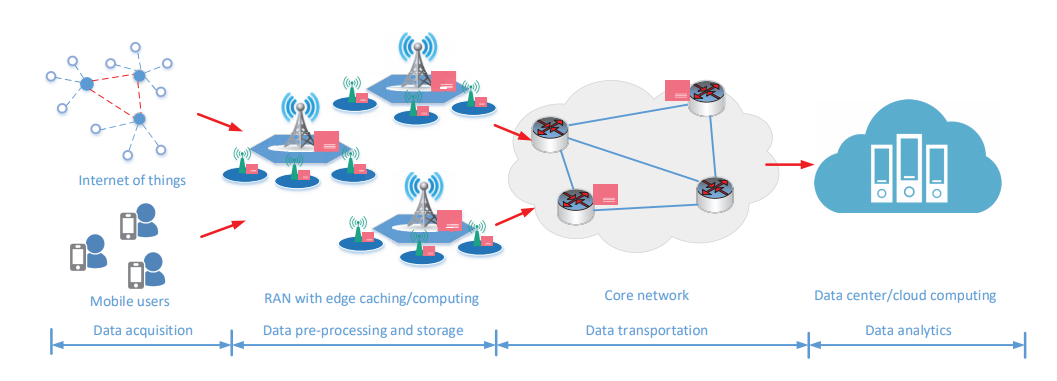
\includegraphics[width=0.4\textwidth]{Capture1.PNG}
\caption{ Big data driven networking}
\label{fig:Bigdata}
\end{figure}

A critical component of network slicing is resource allocation, which needs
to ensure that slices receive the resources needed to support their mobiles/services while optimizing network efficiency.

In a sliced network, network operators
realize the network slices instances to provide the required
network characteristics to different services, pertaining to
third-party tenants.
 Therefore, there will be Service Level
Agreements (SLAs) between network operator and the tenants
to declare the requirements of a particular service and the
operator should fulfill these SLAs via instantiating appropriate
network slices. Requirements of the service instances are
specified in terms of Key Performance Indicators (KPIs), such
as throughput, latency, availability, coverage, etc.

An important aspect of network slicing is to guarantee that
the slices operate independently, i.e., the performance, congestion, failure, etc., in one slice will not negatively influence the
performance of other slices which are sharing the resources.
This means that providing protection from other slices is one to enable Internet of things (IoT) applications, including high data rate, numerous devices
connection and low service latency. Network slicing and fog computing have been envisioned as
promising solutions in service-oriented 5G architecture.

\begin{figure}[h!]
\centering
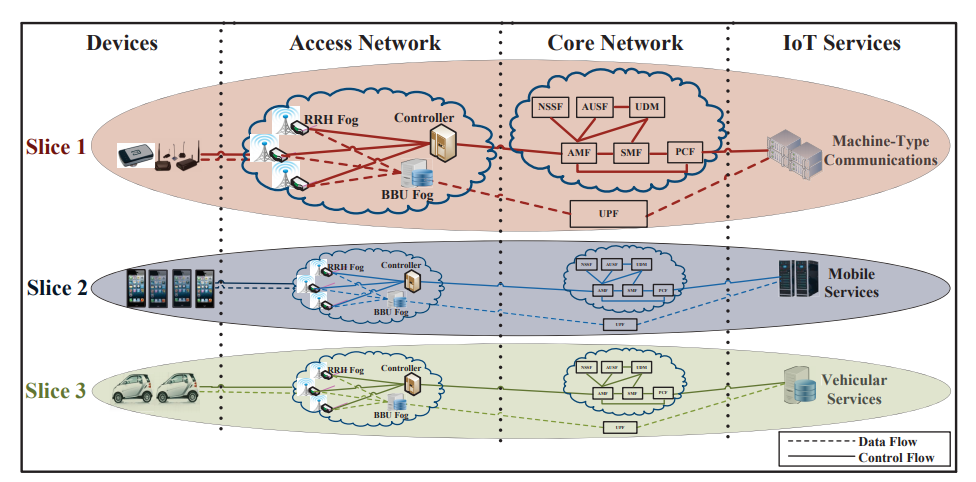
\includegraphics[width=0.4\textwidth]{Capture.PNG}
\caption{ Service-oriented Architecture of Fog-assisted 5G Network with Network Slicing}
\label{fig:FogNS}
\end{figure}

Assume a system model with different types of user equipment (UE).
There exists two different types of
UEs with different requirements: low-latency users (LUs) and
high-data rate Tactile users (TUs).

The first group is very sensitive to the latency. The second group needs high data rate.
Each slice sustains a queue
for the incoming slice traffic, which has a backlog.
%The arrival traffic per slot can be modeled.
The network model is assumed to be composed of a set of M
base stations (BSs).
We have three types of slice resource requirements.
\begin{itemize}
\item A fixed slice requests dedicated radio resources along
time and frequency domains. Therefore, it is isolated
from other slices and does not multiplex its resources
with others. One example is the bandwidth parts (BWPs)
defined in 5G (see 3GPP TS 38.211) that operate on
disjoint parts of the spectrum with a given numerology.
\item A dynamic slice requests a share of resources in terms
of aggregate throughput. It can be mapped to the eMBB
usage scenario, and thus a precise radio resource allocation is less important than the efficient use of available
resources for a guaranteed throughput.
\item An on-demand slice exhibits more stringent requirements
in terms of latency, and hence it can be mapped to
the URLLC scenario. Therefore, such slice should be
assigned radio resources with short delay, in comparison
with the dynamic slice \cite{schmidt2019slice}.
\end{itemize}




\subsection{Introduction to Network slicing}
Network slicing is an important network architecture innovation in 5G that is also expected to be inherited in the next generation. Network slicing enables the coexistence of
multiple isolated and independent virtual (logical) networks,
i.e., slices, on the same physical network infrastructure. The
advantages of network slicing are multifold. First, through the
multiplexing of the virtual networks, network slicing supports
multi-tenancy, i.e., multiple virtual network operators (VNOs)
sharing the same physical network infrastructure. This
reduces capital expense in network deployment and operation. Second, network slicing provides the potential to create customized slices for different service types with various
Quality of Service (QoS) requirements, which can achieve service differentiation
and guarantee service level agreement (SLA) for each service
type. Third, as slices can be created on-demand and modified
or annulled as needed, network slicing increases the flexibility
and adaptability in network management.


A network slice is a virtual network which is implemented on top
of a physical network in a way that creates the illusion to the
slice tenant of operating its own dedicated physical network.
Network Slicing offers a number of significant advantages
that are particularly useful in the design of next generation
wireless networks, namely:
\begin{itemize}
\item  Slice isolation: The complete isolation of slices allows
for a simpler and more efficient design of each slice with
the goal of meeting the requirements of the particular
vertical applications and services offered by the slice
tenant. In addition, network failure, overload, or security
attacks in one slice will not affect the operation of other
slices in the network.
\item Simplified service chains: In contrast to traditional cellular communications in which all services consist of the
same functions, in network slicing each service may rely on a different subset of functions.
\item Flexible VNF placement: NFV introduces an additional
degree of freedom regarding the placement of these functions on the network. Intelligent placement may improve
network performance and reduce operating costs.
\item Transparent slice management: Subsets of the physical
network resources might belong to different network
domains (or even operators). Network Slicing provides
an abstraction of the physical resources and makes slice
management transparent to the slice tenant.
\end{itemize}
We have core and ran slicing in network slicing architecture.
RAN slicing faces the following unique challenges: 
\begin{itemize}
\item 
Resource interplay – Since a service may consume multiple network resources, there exists an inherent tradeoff
among the network resources. For example, in computing offloading services, the service latency consists of
two elements: task transmission latency and task processing latency. If a user associates with a remote MEC
server having abundant computing resources for task
processing, a high task transmission latency will incur.
On the other hand, if a user associates with a nearby
MEC server having insufficient computing resources, it
takes a longer time for task processing. In such a manner, the allocation of computing and communication resources is coupled with each other in the exemplary computing offloading services. Similarly, the allocation of
multiple network resources is intertwined, which complicates the RAN slicing. \textbf{A joint multiple network resource allocation scheme should be judiciously designed
to maximize network welfare.}
\item  Strict QoS requirements – Compared with traditional 4G
networks, 5G networks and beyond have stricter QoS
requirements, including a higher throughput and a lower
latency. Especially, the typical URLLC service in 5G
requires ultra-high reliability (e.g., 99.999), which is
much stricter than that of other services. In addition, the
payload of data packets in URLLC services is usually
small, such as 32 bytes. The transmission performance of short-length packets cannot be characterized
by the traditional Shannon theory which is suitable for
long-length packet transmission due to a large transmission overhead. Instead, the finite block length channel coding theory should be applied to characterize the
achievable rate for short-length packets. Traditional
QoS provisioning is unsuitable for short-length packet
URLLC services with ultra-high reliability. Thus, \textbf{an accurate QoS provisioning for URLLC services is desired
in the RAN slicing framework.}
\item  User mobility – Due to the high network density, users
may frequently move out the coverage of its associated network infrastructure, which results in a dynamic
network topology. For example, high-mobility vehicle
users can trigger handover frequently. The dynamic network topology changes the service traffic distribution,
rendering previously optimal slice allocation suboptimal
over time, degrading network performance, and may
even violate users’ QoS requirements. When the network
performance degrades to a threshold, adjusting existing
slices or creating new slices will be triggered, which
incurs slice reconfiguration overhead. Therefore, \textbf{dynamic yet
efficient RAN slicing to accommodate user mobility remains a challenging issue} \cite{aiNS}.
\end{itemize}

\section{system model and main problem}
In the network slicing architecture, each service is admitted by specific slice. Also each service has a special QoS that must be reached. 
QoS parameters include:

\begin{itemize}
\item Delay
\item Throughput
\item Packet loss
\item Out of order delivery
\end{itemize}  

Different services have one or more of these QoS.
AI-based methods become promising techniques to provide
potential benefits to address the difficulties and complexities of slicing.
We can use AI-based methods
to provide \textbf{accurate service-specific traffic prediction}.
Only
with such accurately predicted service-specific traffic, RAN
slicing can effectively facilitate network resource allocation to
accommodate service demands in the near future. Recent studies show that AI-based methods, such as deep neural network
(DNN) and long short-term memory (LSTM), are capable of
accurately forecasting service-specific traffic load.
AI-based methods can facilitate efficient resource allocation in RAN slicing. An online AI-based resource allocation decision process has the potential to achieve
a low complexity after an offline training procedure, which
addresses the high computational complexity challenge in the
conventional model-based optimization methods.
 Note that traditional RL methods, such as
Q-learning, suffer from the curse of dimensionality, which are
only suitable for RAN slicing problems in small-scale networks. Deep RL methods incorporate deep learning networks
in the RL framework can effectively address the complexity
issues in large-scale networks. 


Cooperative Game with Distributed Learning while existing applications of distributed learning in this field generally consider non-cooperative games where the Nash
equilibriums are achieved, there is a great potential to adopt the concept of cooperative game, where tenants/slices can learn to
make decisions in an organized and cooperative way, in order to maximize the global social welfare instead of their own interests.
In this way, a Pareto optimum can be expected instead of the Nash equilibrium.

\subsection{system model}
In this part, deep reinforcement learning (DRL), which focuses on how to interact with the environment by
trying alternative actions and reinforcing the tendency actions producing more rewarding consequences,
is assumed to be a promising solution for network slicing \cite{drl}.
\begin{figure}%[H]
  \centering
    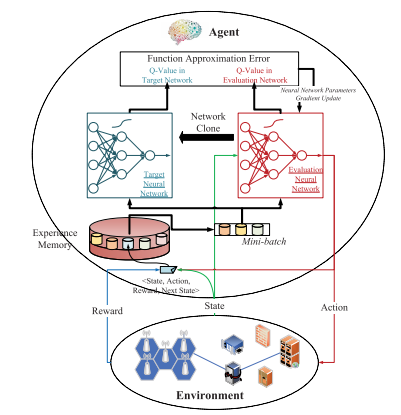
\includegraphics[width=\linewidth]{drl}
  \caption{Deep Q learning structure}
  \label{fig:drl}
\end{figure}
Assume we have $V$ services and $S$ slices. Each service needs physical resource blocks (sharing the aggregated bandwidth $W$), RRHs (radio unit head) and CU (control unit) in RAN and VNFs in core (set of requirements $\mathbf{q} = \{q_1, ..., q_{n_v}\}$) and requests specific QoS includes delay, throughput, packetloss, ... . 
So each service $v$ needs specific demands $\mathbf{d} = \{d_1, ..., d_{n_v}\}$.
The target is to maximize long-term reward expectation $E\{R(\mathbf{q},\mathbf{d})\}$.
\begin{subequations}
\begin{alignat}{4}
\text{argmax}_{\mathbf{d}} E\{R(\mathbf{q},\mathbf{d})\} \\
\text{subject to} \quad  & \mathbf{q} , \mathbf{d}  
\end{alignat}
\label{constraints1}
\end{subequations}
Set of QoSes $\mathbf{d} = \{d_1, ..., d_{n_v}\}$ includes M/M/1 delays, throughput and packetloss.
\begin{figure}%[H]
  \centering
    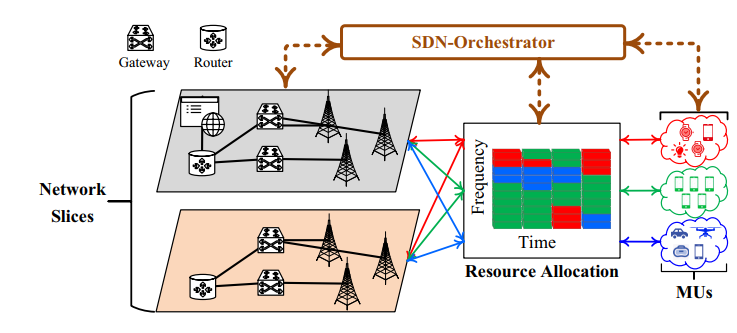
\includegraphics[width=\linewidth]{NS}
  \caption{Network slicing structure \cite{gan}}
  \label{fig:NS}
\end{figure}
\subsubsection{Delay}
Assume the packet arrival of UEs follows a Poisson process with arrival rate $\lambda_v$ for the  UEs of the $v^{th}$ service.
Therefore, the mean arrival data rate of UEs is
\begin{equation}
D_{v} = \frac{1}{\mu - \lambda_v}.
\end{equation}
where $1/\mu$ is the mean service time and $\lambda$ is the rate of arrival packets.
\subsubsection{Throughput}
Let $\rho_v$ be the mean downlink rate of user $i$ served by service $v$, which
is, for simplicity, defined by Shannon theory as follows
\begin{equation}
\rho_v = w_v log(1+\frac{P_v}{N_v}) 
\end{equation}
where $w_v$ is the bandwidth of service $v$.
\bibliographystyle{IEEEtran}
\bibliography{references}
\end{document} 